\chapter{Avaliação} \label{chap:resultados}

\section{Coleções de dados} \label{sec:colecoes}

A evolução do estado da arte do reconhecimento facial automático em imagens tem beneficiado em larga escala do aumento constante dos recursos disponíveis para o seu estudo, nomeadamente através da criação de novas e mais completas coleções de dados \cite{Huang2007}. A grande maioria destas coleções, caracteriza-se por ter condições de captura controladas com o intuito de efetuar o estudo de fatores específicos que afetam a qualidade do reconhecimento, tais como a variação da pose, iluminação, expressão e outros fatores mencionados no capítulo \ref{desafios}. O objeto de estudo desta dissertação não é, no entanto, a análise específica de alguns desses fatores, mas sim do impacto do uso de abstração de imagens em todo o processo de reconhecimento facial. Desta forma, a escolha de uma biblioteca apropriada e que represente as grandes variações associadas aos diferentes desafios que afetam o reconhecimento facial em imagens torna-se crucial.

Tendo em conta as preocupações acima mencionadas, para a análise dos resultados obtidos do trabalho realizado no âmbito nesta dissertação foi escolhida a coleção de imagens \textit{Labeled Faces in the Wild}. Esta coleção é constituída por um conjunto de imagens faciais e respetivas anotações textuais e encontra-se descrita em maior pormenor na secção seguinte deste documento.

Para um estudo científico e rigoroso do impacto dos filtros de abstração no reconhecimento facial, para além da escolha de um conjunto de dados a analisar, torna-se também importante a construção de sub-conjuntos de teste, assim como a definição de uma metodologia de avaliação adequada. Na secção \ref{sec:conjuntos} encontram-se detalhados os conjuntos de teste criados e nas secções \ref{falta} e \ref{falta} as metodologias de avaliação adotadas.

\subsection{\textit{Labeled Faces in the Wild}}  \label{sec:lfw}
A coleção \textit{Labeled Faces in the Wild (LFW)} é uma base de dados fotográfica desenhada especificamente para o estudo do problema de reconhecimento facial, particularmente em situações onde as condições de captura das imagens não possuem restrições. Nesse sentido, as imagens que constituem a galeria caracterizam-se por possuir uma grande variabilidade, nomeadamente ao nível da pose, expressão, iluminação, etnia, idade, género, vestuário e qualidade da câmara, por exemplo \cite{Huang2007}.

Nesta coleção encontram-se representados um conjunto de 5749 indivíduos, ilustrados por 13233 imagens. O número de imagens por pessoa apresenta no entanto uma grande variação, desde um mínimo de 1 imagem por pessoa para 4069 indivíduos, até um máximo de 530 imagens que representam o antigo presidente dos Estados Unidos da América George W. Bush. A distribuição do número de imagens por pessoa poderá ser consultada com mais detalhe na figura \ref{fig:distribuicaoLFW}.

\begin{figure}[ht]
  \begin{center}
    \leavevmode
    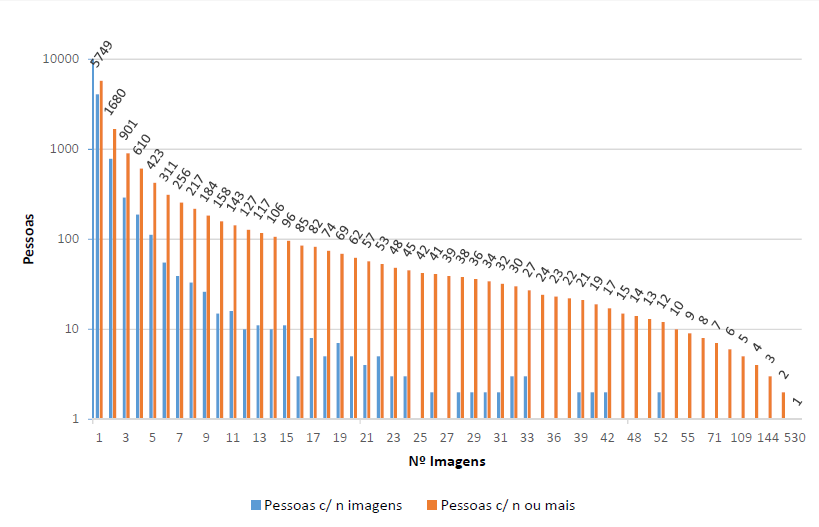
\includegraphics[width=1\textwidth]{Distribuicao}
    \caption{Distribuição do número de imagens por pessoa na biblioteca LFW.}
    \label{fig:distribuicaoLFW}
  \end{center}
\end{figure}

Para além da distribuição do número de imagens por pessoa, as restantes características da biblioteca LFW encontram-se resumidas na tabela \ref{tab:lfw}. As imagens são maioritariamente a cores, com diferentes graus de saturação e devido à inexistência de restrições de captura de imagens, cada fotografia pode possuir mais do que uma face representada, sendo que a face que contem o pixel central deve ser considerada como a entidade representada na imagem. A cada imagem encontra-se também associada uma anotação textual, relativa ao nome da pessoa representada. 
\begin{center}
\begin{table}
	\caption{Caracterização da Biblioteca LFW}
	\begin{center}
    \begin{tabular}{ll}
    \hline
    Característica                            & Valor            \\ \hline
    Imagens                                   & 13233 imagens    \\
    Pessoas representadas                     & 5749 pessoas     \\
    Tamanho total / Formato                   & 179 MB / JPEG    \\
    Tamanho de cada imagem: min / médio / max & ~                \\
    Dimensões imagem                          & 250 $x$ 250 pixeis \\
    \hline
    \end{tabular}
	\label{tab:lfw}
	\end{center}
\end{table}
\end{center}

Esta biblioteca é particularmente interessante para o estudo do desempenho do sistema desenvolvido e consequentemente do impacto do uso da abstração de imagens no reconhecimento facial uma vez que a variabilidade presente nas suas imagens, representa uma amostra fiável das variações encontradas no dia-a-dia de uma pessoa. Por outro lado, o facto de as suas imagens não terem sido capturadas com o intuito específico da análise do problema do reconhecimento facial, aproxima este conjunto de dados das imagens utilizadas por um utilizador final de um sistema de reconhecimento facial automático. Finalmente, o facto de esta coleção já ter sido pré-processada de modo a se encontrar preparada especificamente para o estudo do desempenho de sistemas de reconhecimento facial automático permitiu agilizar os testes efetuados.

\subsection{Pré-processamento}  \label{sec:preprocessamento}
... refazer isto...
Para além da coleção LFW original, encontram-se também disponíveis para fins de investigação duas outras coleções derivadas da coleção original, com as mesmas imagens, mas onde estas foram sujeitas a um pré-processamento com vista a efetuar o alinhamento da posição da face na imagem. Uma vez que a tarefa de alinhamento da face na imagem não é um objeto de estudo primordial desta dissertação optamos pela utilização da versão alinhada LFW-a \citep{autor} para fins de avaliação do desempenho do sistema de reconhecimento facial criado e do impacto do uso de filtros de abstração sobre essas imagens.

O conjunto de imagens que constituem a biblioteca LFW-a foi ainda sujeito a um conjunto de tarefas de pré-processamento com vista a melhorar a eficácia do reconhecimento assim como analisar o impacto dos diferentes pré-processamentos na resolução do problema de reconhecimento facial automático. A cadeia de pré-processamento é constituída por quatro passos, tal como pode ser visualizado na figura \ref{fig:preprocessamento}, sendo que apenas o primeiro é obrigatório para todas as imagens pré-processadas.

\begin{figure}[ht]
  \begin{center}
    \leavevmode
    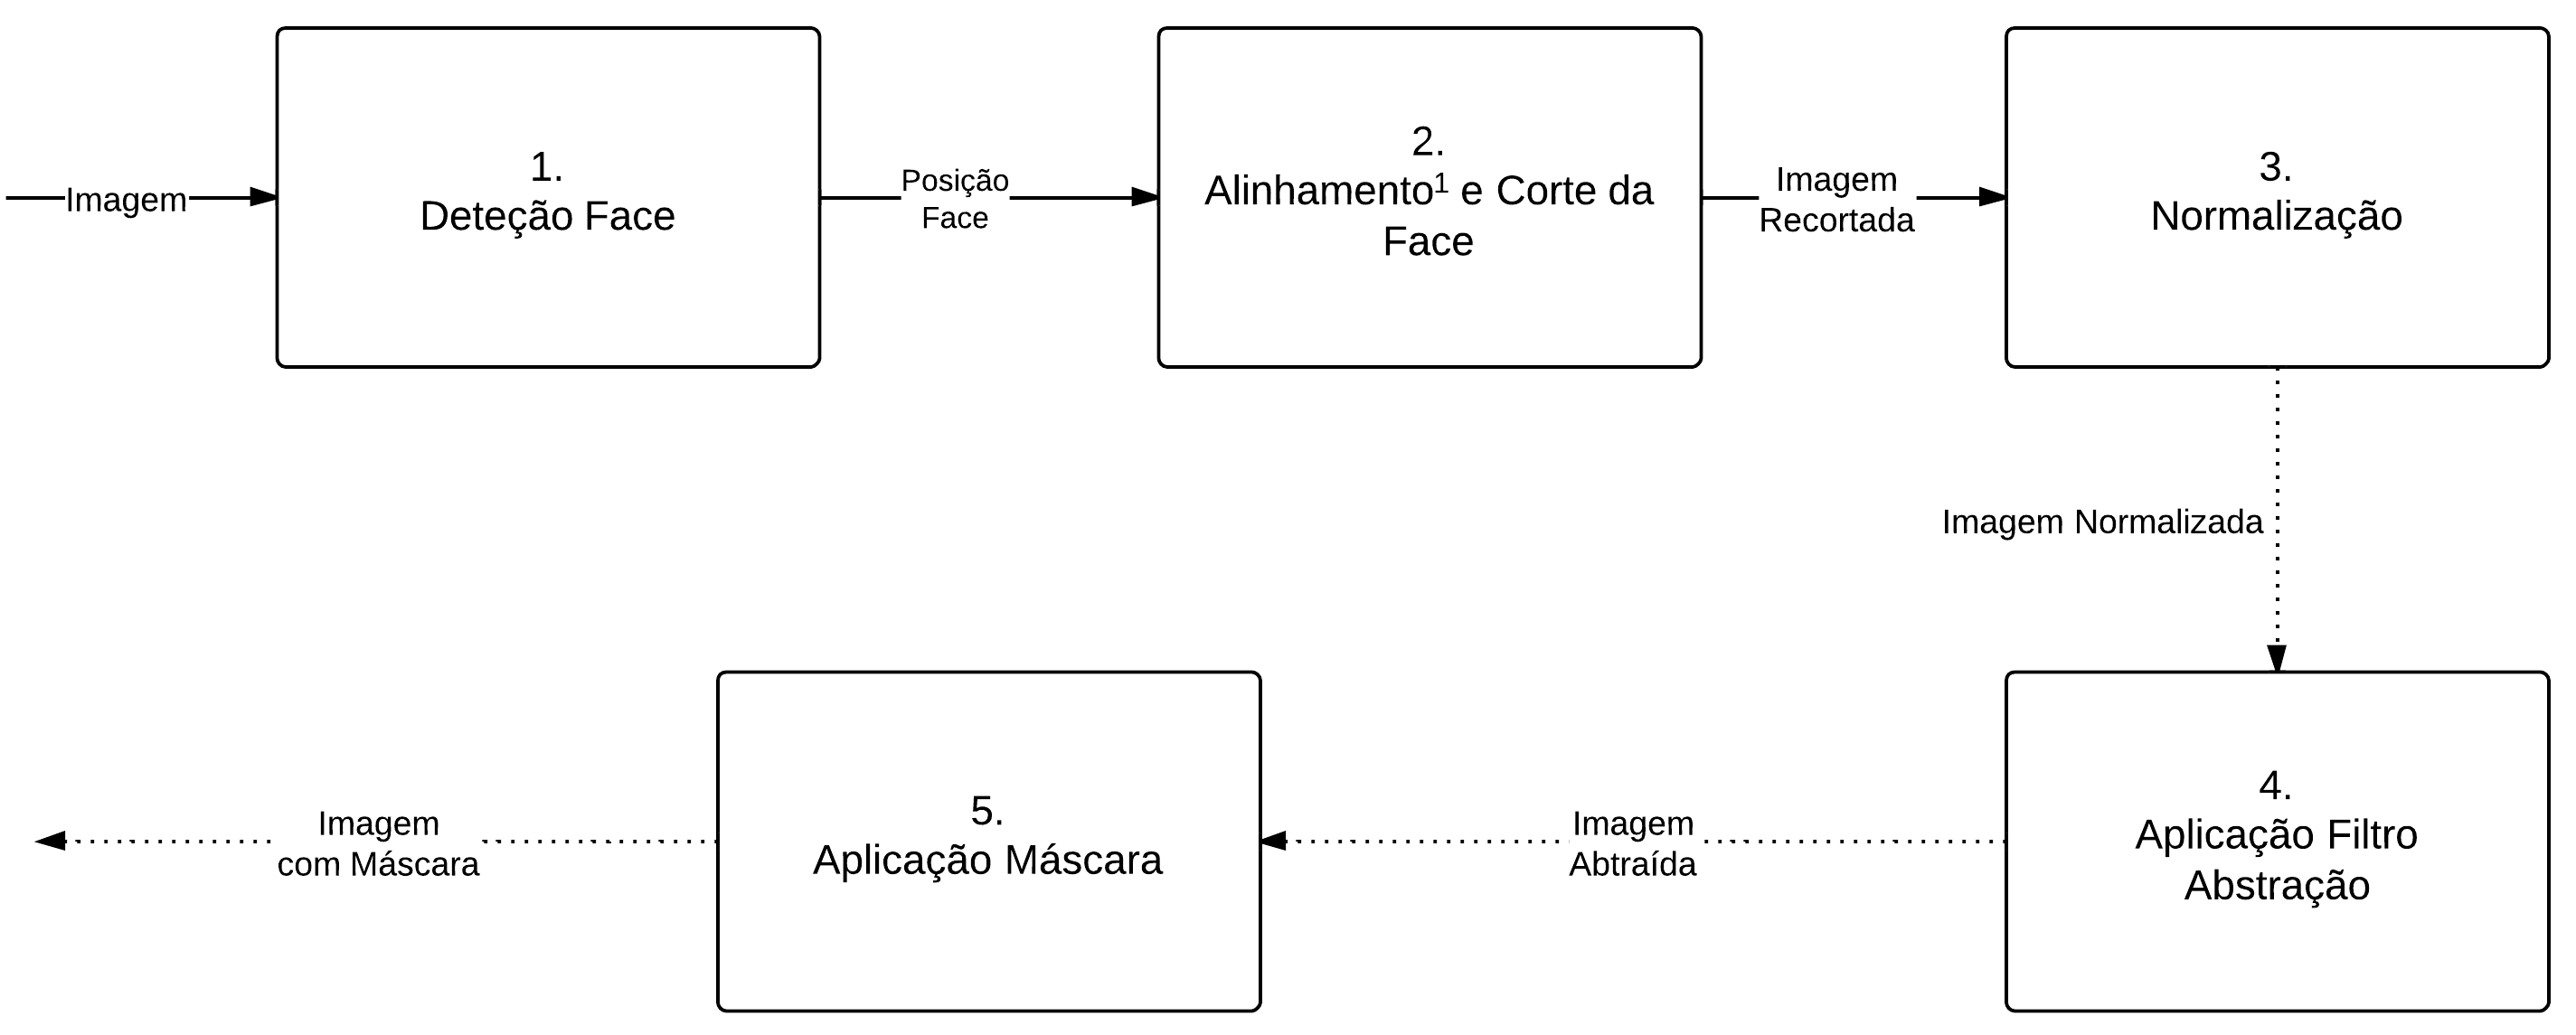
\includegraphics[width=0.7\textwidth]{PreProcessamentoVisage}
    \caption{Cadeia de pré-processamento a que as imagens foram sujeitas.}
    \label{fig:preprocessamento}
  \end{center}
\end{figure}

O passo 1 é responsável pela deteção da localização da face na imagem e efetuar a respectiva segmentação da mesma, de acordo com descrito em \ref{chap:detector}. Após a obtenção da face extraída da imagem é então possível proceder à sua normalização em termos de contraste. Para isso foram analisadas três possibilidades: \textit{contrast streching}, \textit{histogram equalization} e ainda \textit{CLAHE}. Posteriormente a imagem po....

\begin{center}
\begin{table}
	\caption{Sub-coleções criadas após pré-processamento.}
	\begin{center}
    \begin{tabular}{llllll}
    \hline
    Designação & Coleção Original & Recortada & Normalização           & Filtro Abstração & Máscara \\
    Original   & LFW-a            & -         & -                      & -                & -       \\
    Cropped    & LFW-a            & X         & -                      & -                & -       \\
    Masked     & LFW-a            & X         & -                      & -                & X       \\
    Normalized & LFW-a            & X         & Constrast Streching    & -                & X       \\
    Equalized  & LFW-a            & X         & Histogram Equalization & -                & X       \\
    CLAHE      & LFW-a            & X         & CLAHE                  & -                & X       \\
    Bilateral  & LFW-a            & X         & Histogram Equalization & Bilateral Filter & X       \\
    Gaussian   & LFW-a            & X         & Histogram Equalization & Gaussian Filter  & X       \\
    \hline
    \end{tabular}
	\label{tab:colecoes}
	\end{center}
\end{table}
\end{center}

\subsection{Conjuntos de Teste}  \label{sec:conjuntos}
O desempenho de sistemas de reconhecimento facial pode ser analisado através de diferentes perspetivas, tal como introduzido no capítulo \ref{chap:problema} desta dissertação. A biblioteca LFW foi criada com o propósito inicial da análise do sub-problema de reconhecimento facial \textit{pair matching}, no qual o sistema deve decidir se duas faces representam ou não o mesmo indivíduo. No entanto, as características desta biblioteca, nomeadamente no que diz respeito à existência da anotação textual das pessoas presentes em cada imagem, à existência de apenas uma pessoa representada em cada imagem e ainda da normalização do formato das imagens, permitem que esta biblioteca possa ser utilizada com um esforço reduzido para o analise dos restantes sub-problemas de reconhecimento facial automático.

-No âmbito desta dissertação temos em vista a análise da desempenho do reconhecimento através de duas perspetivas descritas nos pontos \ref{sec:avaliacao1} e \ref{sec:avaliacao2} a seguir. Uma vez que estas avaliações não se encontram enquadradas no paradigma de avaliação de \textit{pair matching} foi necessário a criação de novos conjuntos de teste. 

Desta forma foram criados 4 conjuntos de teste
- cada um com
	Total Images: 1180
	Total People: 59
	16 treino, 4 de teste
	
A diferença entre os vários conjuntos são as imagens de treino e as de teste, desta forma é possível analisar a variação da performance do sistema nos 6 conjuntos.


\section{Avaliação do desempenho em Identificação Ranking N} \label{sec:avaliacao1}
Medida padrão de avaliação de reconhecimento facial
Usada em várias avaliações efetuadas, desde a mais antiga FRVT até à recente MBE 2010

\subsection{Metodologias Avaliação}

\subsection{Resultados}

\section{Avaliação do desempenho em Retrieval} \label{sec:avaliacao2}

\subsection{Metodologias Avaliação}

\subsection{Resultados}

